\documentclass[11pt,a4paper,]{article}
\usepackage{lmodern}

\usepackage{amssymb,amsmath}
\usepackage{ifxetex,ifluatex}
\usepackage{fixltx2e} % provides \textsubscript
\ifnum 0\ifxetex 1\fi\ifluatex 1\fi=0 % if pdftex
  \usepackage[T1]{fontenc}
  \usepackage[utf8]{inputenc}
\else % if luatex or xelatex
  \usepackage{unicode-math}
  \defaultfontfeatures{Ligatures=TeX,Scale=MatchLowercase}
\fi
% use upquote if available, for straight quotes in verbatim environments
\IfFileExists{upquote.sty}{\usepackage{upquote}}{}
% use microtype if available
\IfFileExists{microtype.sty}{%
\usepackage[]{microtype}
\UseMicrotypeSet[protrusion]{basicmath} % disable protrusion for tt fonts
}{}
\PassOptionsToPackage{hyphens}{url} % url is loaded by hyperref
\usepackage[unicode=true]{hyperref}
\hypersetup{
            pdftitle={A fast and elegant method for forecast reconciliation using linear forecasting models},
            pdfkeywords={hierarchical forecasting, grouped forecasting, reconciling forecast,
linear regression},
            pdfborder={0 0 0},
            breaklinks=true}
\urlstyle{same}  % don't use monospace font for urls
\usepackage{geometry}
\geometry{left=2.5cm,right=2.5cm,top=2.5cm,bottom=2.5cm}
\usepackage[style=authoryear-comp,]{biblatex}
\addbibresource{references.bib}
\usepackage{longtable,booktabs}
% Fix footnotes in tables (requires footnote package)
\IfFileExists{footnote.sty}{\usepackage{footnote}\makesavenoteenv{long table}}{}
\IfFileExists{parskip.sty}{%
\usepackage{parskip}
}{% else
\setlength{\parindent}{0pt}
\setlength{\parskip}{6pt plus 2pt minus 1pt}
}
\setlength{\emergencystretch}{3em}  % prevent overfull lines
\providecommand{\tightlist}{%
  \setlength{\itemsep}{0pt}\setlength{\parskip}{0pt}}
\setcounter{secnumdepth}{5}

% set default figure placement to htbp
\makeatletter
\def\fps@figure{htbp}
\makeatother


\title{A fast and elegant method for forecast reconciliation using linear
forecasting models}

%% MONASH STUFF

%% CAPTIONS
\RequirePackage{caption}
\DeclareCaptionStyle{italic}[justification=centering]
 {labelfont={bf},textfont={it},labelsep=colon}
\captionsetup[figure]{style=italic,format=hang,singlelinecheck=true}
\captionsetup[table]{style=italic,format=hang,singlelinecheck=true}

%% FONT
\RequirePackage{bera}
\RequirePackage{mathpazo}

%% HEADERS AND FOOTERS
\RequirePackage{fancyhdr}
\pagestyle{fancy}
\rfoot{\Large\sffamily\raisebox{-0.1cm}{\textbf{\thepage}}}
\makeatletter
\lhead{\textsf{\expandafter{\@title}}}
\makeatother
\rhead{}
\cfoot{}
\setlength{\headheight}{15pt}
\renewcommand{\headrulewidth}{0.4pt}
\renewcommand{\footrulewidth}{0.4pt}
\fancypagestyle{plain}{%
\fancyhf{} % clear all header and footer fields
\fancyfoot[C]{\sffamily\thepage} % except the center
\renewcommand{\headrulewidth}{0pt}
\renewcommand{\footrulewidth}{0pt}}

%% MATHS
\RequirePackage{bm,amsmath}
\allowdisplaybreaks

%% GRAPHICS
\RequirePackage{graphicx}
\setcounter{topnumber}{2}
\setcounter{bottomnumber}{2}
\setcounter{totalnumber}{4}
\renewcommand{\topfraction}{0.85}
\renewcommand{\bottomfraction}{0.85}
\renewcommand{\textfraction}{0.15}
\renewcommand{\floatpagefraction}{0.8}

%\RequirePackage[section]{placeins}

%% SECTION TITLES
\RequirePackage[compact,sf,bf]{titlesec}
\titleformat{\section}[block]
  {\fontsize{15}{17}\bfseries\sffamily}
  {\thesection}
  {0.4em}{}
\titleformat{\subsection}[block]
  {\fontsize{12}{14}\bfseries\sffamily}
  {\thesubsection}
  {0.4em}{}
\titlespacing{\section}{0pt}{*5}{*1}
\titlespacing{\section}{0pt}{*2}{*0.2}


%% TITLE PAGE
\def\Date{\number\day}
\def\Month{\ifcase\month\or
 January\or February\or March\or April\or May\or June\or
 July\or August\or September\or October\or November\or December\fi}
\def\Year{\number\year}

\makeatletter
\def\wp#1{\gdef\@wp{#1}}\def\@wp{??/??}
\def\jel#1{\gdef\@jel{#1}}\def\@jel{??}
\def\showjel{{\large\textsf{\textbf{JEL classification:}}~\@jel}}
\def\nojel{\def\showjel{}}
\def\addresses#1{\gdef\@addresses{#1}}\def\@addresses{??}
\def\cover{{\sffamily\setcounter{page}{0}
        \thispagestyle{empty}%
        \vspace*{-2cm}
        \centerline{\raisebox{-1.8cm}{
\includegraphics[width=5cm]{MBSportrait}}\hspace*{9cm} ISSN 1440-771X}\vspace{0.99cm}
        \begin{center}\Large
        Department of Econometrics and Business Statistics\\[.5cm]
        \scriptsize http://business.monash.edu/econometrics-and-business-statistics/research/publications
        \end{center}\vspace{2cm}
        \begin{center}
        \fbox{\parbox{14cm}{\begin{onehalfspace}\centering\Huge\vspace*{0.3cm}
                \textsf{\textbf{\expandafter{\@title}}}\vspace{1cm}\par
                \LARGE\@author\end{onehalfspace}
        }}
        \end{center}
        \vfill
                \begin{center}\Large
                \Month~\Year\\[1cm]
                Working Paper \@wp
        \end{center}}}
\def\pageone{{\sffamily\setstretch{1}%
        \thispagestyle{empty}%
        \vbox to \textheight{%
        \raggedright\baselineskip=1.2cm
     {\fontsize{24.88}{30}\sffamily\textbf{\expandafter{\@title}}}
        \vspace{2cm}\par
        \hspace{1cm}\parbox{14cm}{\sffamily\large\@addresses}\vspace{1cm}\vfill
        \hspace{1cm}{\large\Date~\Month~\Year}\\[1cm]
        \hspace{1cm}\showjel\vss}}}
\def\blindtitle{{\sffamily
     \thispagestyle{plain}\raggedright\baselineskip=1.2cm
     {\fontsize{24.88}{30}\sffamily\textbf{\expandafter{\@title}}}\vspace{1cm}\par
        }}
\def\titlepage{{\cover\newpage\pageone\newpage\blindtitle}}

\def\blind{\def\titlepage{{\blindtitle}}\let\maketitle\blindtitle}
\def\titlepageonly{\def\titlepage{{\pageone\end{document}}}}
\def\nocover{\def\titlepage{{\pageone\newpage\blindtitle}}\let\maketitle\titlepage}
\let\maketitle\titlepage
\makeatother

%% SPACING
\RequirePackage{setspace}
\spacing{1.5}

%% LINE AND PAGE BREAKING
\sloppy
\clubpenalty = 10000
\widowpenalty = 10000
\brokenpenalty = 10000
\RequirePackage{microtype}

%% PARAGRAPH BREAKS
\setlength{\parskip}{1.4ex}
\setlength{\parindent}{0em}

%% HYPERLINKS
\RequirePackage{xcolor} % Needed for links
\definecolor{darkblue}{rgb}{0,0,.6}
\RequirePackage{url}

\makeatletter
\@ifpackageloaded{hyperref}{}{\RequirePackage{hyperref}}
\makeatother
\hypersetup{
     citecolor=0 0 0,
     breaklinks=true,
     bookmarksopen=true,
     bookmarksnumbered=true,
     linkcolor=darkblue,
     urlcolor=blue,
     citecolor=darkblue,
     colorlinks=true}

%% KEYWORDS
\newenvironment{keywords}{\par\vspace{0.5cm}\noindent{\sffamily\textbf{Keywords:}}}{\vspace{0.25cm}\par\hrule\vspace{0.5cm}\par}

%% ABSTRACT
\renewenvironment{abstract}{\begin{minipage}{\textwidth}\parskip=1.4ex\noindent
\hrule\vspace{0.1cm}\par{\sffamily\textbf{\abstractname}}\newline}
  {\end{minipage}}


\usepackage[T1]{fontenc}
\usepackage[utf8]{inputenc}

\usepackage[showonlyrefs]{mathtools}
\usepackage[no-weekday]{eukdate}

%% BIBLIOGRAPHY

\makeatletter
\@ifpackageloaded{biblatex}{}{\usepackage[style=authoryear-comp, backend=biber, natbib=true]{biblatex}}
\makeatother
\ExecuteBibliographyOptions{bibencoding=utf8,minnames=1,maxnames=3, maxbibnames=99,dashed=false,terseinits=true,giveninits=true,uniquename=false,uniquelist=false,doi=false, isbn=false,url=true,sortcites=false}

\DeclareFieldFormat{url}{\texttt{\url{#1}}}
\DeclareFieldFormat[article]{pages}{#1}
\DeclareFieldFormat[inproceedings]{pages}{\lowercase{pp.}#1}
\DeclareFieldFormat[incollection]{pages}{\lowercase{pp.}#1}
\DeclareFieldFormat[article]{volume}{\mkbibbold{#1}}
\DeclareFieldFormat[article]{number}{\mkbibparens{#1}}
\DeclareFieldFormat[article]{title}{\MakeCapital{#1}}
\DeclareFieldFormat[article]{url}{}
%\DeclareFieldFormat[book]{url}{}
%\DeclareFieldFormat[inbook]{url}{}
%\DeclareFieldFormat[incollection]{url}{}
%\DeclareFieldFormat[inproceedings]{url}{}
\DeclareFieldFormat[inproceedings]{title}{#1}
\DeclareFieldFormat{shorthandwidth}{#1}
%\DeclareFieldFormat{extrayear}{}
% No dot before number of articles
\usepackage{xpatch}
\xpatchbibmacro{volume+number+eid}{\setunit*{\adddot}}{}{}{}
% Remove In: for an article.
\renewbibmacro{in:}{%
  \ifentrytype{article}{}{%
  \printtext{\bibstring{in}\intitlepunct}}}

\AtEveryBibitem{\clearfield{month}}
\AtEveryCitekey{\clearfield{month}}

\makeatletter
\DeclareDelimFormat[cbx@textcite]{nameyeardelim}{\addspace}
\makeatother
\renewcommand*{\finalnamedelim}{%
  %\ifnumgreater{\value{liststop}}{2}{\finalandcomma}{}% there really should be no funny Oxford comma business here
  \addspace\&\space}


\wp{no/yr}
\jel{C10,C14,C22}

\nocover

\author{Mahsa~Ashouri, Rob J~Hyndman, Galit~Shmueli}
\addresses{\textbf{Mahsa Ashouri}\newline
Institute of Service Science, National Tsing Hua University, Taiwan
\newline{Email: \href{mailto:mahsa.ashouri@iss.nthu.edu.tw}{\nolinkurl{mahsa.ashouri@iss.nthu.edu.tw}}}\newline Corresponding author\\[1cm]
\textbf{Rob J Hyndman}\newline
Monash University, Clayton VIC 3800, Australia
\newline{Email: \href{mailto:rob.hyndman@monash.edu}{\nolinkurl{rob.hyndman@monash.edu}}}\\[1cm]
\textbf{Galit Shmueli}\newline
Institute of Service Science, National Tsing Hua University, Taiwan
\newline{Email: \href{mailto:galit.shmueli@iss.nthu.edu.tw}{\nolinkurl{galit.shmueli@iss.nthu.edu.tw}}}\\[1cm]
}

\date{\sf\Date~\Month~\Year}
\makeatletter
 \lfoot{\sf Ashouri, Hyndman, Shmueli: \@date}
\makeatother

%% Any special functions or other packages can be loaded here.

\usepackage{booktabs}
\usepackage{float}
\usepackage{longtable}
\usepackage{cases}
\usepackage{array}
\usepackage{todonotes}
%\usepackage[backend=biber]{biblatex}
%\usepackage[backend=biber, bibencoding=utf8, style=authoryear, citestyle=authoryear]{biblatex}

\mathtoolsset{showonlyrefs=true}
\allowdisplaybreaks

\def\addlinespace{}
\usepackage[section]{placeins}

\usepackage{float}
\let\origfigure\figure
\let\endorigfigure\endfigure
\renewenvironment{figure}[1][2] {
    \expandafter\origfigure\expandafter[!htbp]
} {
    \endorigfigure
}

\let\origtable\table
\let\endorigtable\endtable
\renewenvironment{table}[1][2] {
    \expandafter\origtable\expandafter[!htbp]
} {
    \endorigtable
}


\begin{document}
\maketitle
\begin{abstract}
Forecasting hierarchical or grouped time series involves two steps:
computing base forecasts and reconciling the forecasts. Base forecasts
can be computed by popular time series forecasting methods such as
Exponential Smoothing (ETS) and Autoregressive Integrated Moving Average
(ARIMA) models. The reconciliation step is a linear process that adjusts
the base forecasts to ensure they are coherent. However using ETS or
ARIMA for base forecasts can be computationally challenging when there
are a large number of series to forecast, as each model must be
numerically optimized for each series. We propose a linear model that
avoids this computational problem. The proposed method is very flexible
in incorporating external data, handling missing values and model
selection. We illustrate our approach using two datasets: monthly
Australian domestic tourism and daily Wikipedia pageviews. We compare
our approach to reconciliation using ETS and ARIMA, and show that our
approach is much faster while providing similar levels of forecast
accuracy.
\end{abstract}
\begin{keywords}
hierarchical forecasting, grouped forecasting, reconciling forecast,
linear regression
\end{keywords}

\hypertarget{introduction}{%
\section{Introduction}\label{introduction}}

Modern data collection tools have dramatically increased the amount of
available time series data. For example, the Internet of Things and
point-of-sale scanning produce huge volumes of time series in a short
period of time. Naturally, there is an interest in forecasting these
time series, yet forecasting large collections of time series is
computationally challenging.

\hypertarget{hierarchical-and-grouped-time-series}{%
\subsection{Hierarchical and grouped time
series}\label{hierarchical-and-grouped-time-series}}

In many cases, these time series can be structured and disaggregated
based on hierarchies or groups such as geographic location, product
type, gender, etc. An example of hierarchical time series is sales in
restaurant chains, which can be disaggregated into different stores and
then different types of food or drinks. Figure
\ref{fig:hierarchicalexample} shows a schematic of such a hierarchical
time series structure with three levels. The top level (level 0) is the
total series, formed by aggregating all the bottom level series. In the
middle level (level 1), series are aggregations of their own child
series; for instance, series A is the aggregation of AW and AX. Finally,
the bottom level series (level 2), includes the most disaggregated
series.

\begin{figure}

{\centering 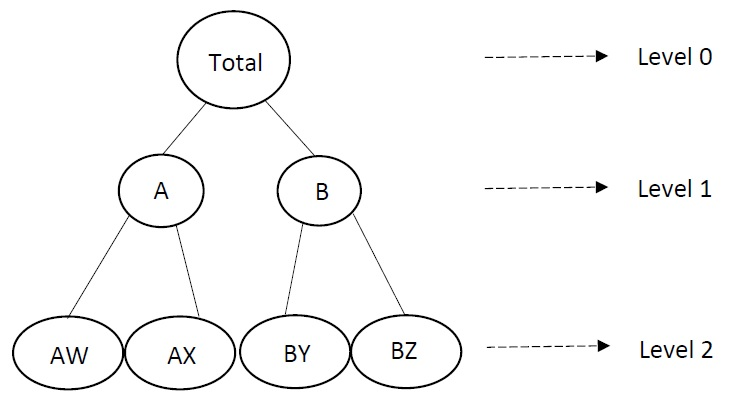
\includegraphics[width=280px,height=170px]{Paper-Figures/hierarchical_example} 

}

\caption{An example of a two level hierarchical structure.}\label{fig:hierarchicalexample}
\end{figure}

Grouped time series involve more complicated aggregation structures
compared to strictly hierarchical time series. To take the simplest
example, suppose we have two grouping factors which are not nested: sex
(Male/Female) and city (New York/San Francisco). The disaggregated
series for each combination of sex and city can be combined to form city
sub-totals, or sex sub-totals. These sub-totals can be combined to give
the overall total. Both sub-totals are of interest.

We can think of such structures as hierarchical time series without a
unique hierarchy. A schematic of this grouped time series structure is
shown in Figure \ref{fig:groupexample} with two grouping factors, each
of two levels (A/B and C/D). The series in this structure can be split
first into groups A and B and then subdivided further into C and D (left
side), or split first into C and D and then subdivided into A and B
(right side). The final disaggregation is identical in both cases, but
the middle level aggregates are different.

\begin{figure}

{\centering 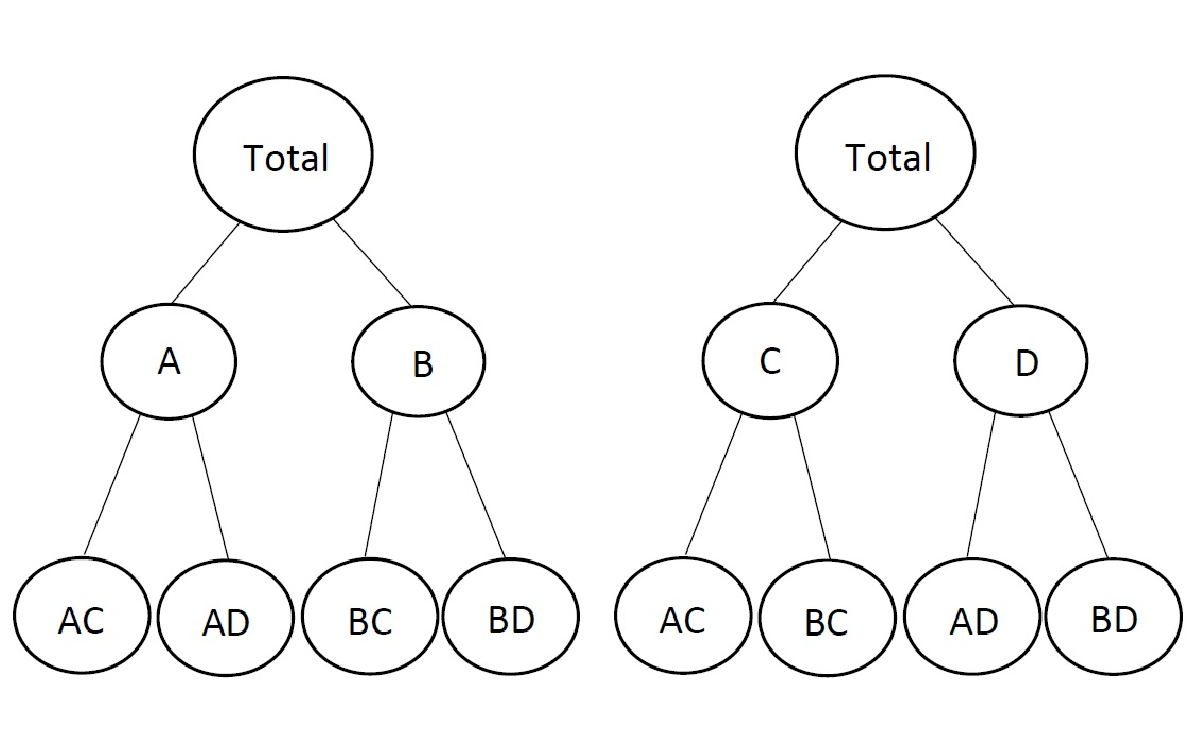
\includegraphics[width=330px,height=180px]{hcf_files/figure-latex/groupexample-1} 

}

\caption{An example of a two level grouped structure.}\label{fig:groupexample}
\end{figure}

We use the same notation \autocite[following][]{fpp2} for both
hierarchical and grouped time series. We denote the total series at time
\(t\) by \(y_t\), and the series at node \(Z\) (subaggregation level
\(Z\)) and time \(t\) by \(y_{Z,t}\). For describing the relationships
between series, we use an \(n\times m\) matrix, called the `summing
matrix', denoted by \(\bm{S}\), in which \(n\) is the overall number of
nodes and \(m\) is the number of bottom level nodes. For example in
Figure \ref{fig:hierarchicalexample}, \(n = 7\) and \(m = 4\), while in
Figure \ref{fig:groupexample}, \(n=9\) and \(m=4\). Then we can write
\(\bm{y}_t=\bm{S}\bm{b}_t\), where \(\bm{y}_t\) is a vector of all the
level nodes at time \(t\) and \(\bm{b}_t\) is the vector of all the
bottom level nodes at time \(t\). For the example shown in Figure
\ref{fig:groupexample}, the equation can be written as follows:
\begin{equation}\label{eq:Smatrixexample}
\begin{pmatrix}
  y_{t}\\y_{A,t}\\y_{B,t}\\y_{C,t}\\y_{D,t}\\y_{AC,t}\\y_{AD,t}\\y_{BC,t}\\y_{BD,t}
\end{pmatrix} =
\begin{pmatrix}
  1&1&1&1\\1&1&0&0\\0&0&1&1\\1&0&1&0\\0&1&0&1\\1&0&0&0\\0&1&0&0\\0&0&1&0\\0&0&0&1\\
\end{pmatrix}
\begin{pmatrix}
  y_{AC,t}\\y_{AD,t}\\y_{BC,t}\\y_{BD,t}\\
\end{pmatrix}.
\end{equation}

\hypertarget{forecasting-hierarchical-time-series}{%
\subsection{Forecasting hierarchical time
series}\label{forecasting-hierarchical-time-series}}

If we just forecast each series individually, we are ignoring the
hierarchical or grouping structure, and the forecasts will not be
``coherent'' (they will not add up appropriately).

There are several available methods that consider the hierarchical
structure information when forecasting time series. These include the
top-down \autocite{gross1990disaggregation,fliedner2001hierarchical},
bottom-up \autocite{kahn1998revisiting}, middle-out and optimal
combination \autocite{hyndman2011optimal} approaches. In the top-down
approach, we first forecast the total series and then disaggregate the
forecast to form lower level series forecasts based on a set of
historical and forecasted proportions \autocite[for details
see][]{athanasopoulos2009hierarchical}. In the bottom-up approach, the
forecasts in each level of the hierarchy can be computed by aggregating
the bottom level series forecasts. However, we may not get good
upper-level forecasts because the most disaggregated series can be noisy
and so their forecasts are often inaccurate. In the middle-out approach,
the process can be started from one of the middle levels and other
forecasts can be computed using aggregation for upper levels and
disaggregation for lower levels. Finally, optimal combination uses all
the \(n\) forecasts for all of the series in the entire structure, and
then uses an optimization process to reconcile the resulting forecasts.
The advantage of the optimal combination method, compared with the other
methods, is that it considers all information in the hierarchy,
including any correlations among the series.

In the optimal combination method, reconciled forecasts can be computed
using the following equeation known as weighted least squares (WLS)
\autocite{mint2018}

\begin{equation}\label{eq:mint}
  \tilde{\bm{y}}_{h}=\bm{S}(\bm{S}'\bm{W}_h^{-1}\bm{S})^{-1}\bm{S}'\bm{W}_h^{-1}\hat{\bm{y}}_h,
\end{equation}

where \(\hat{\bm{y}}_h\) represents a vector of \(h\)-step-ahead base
forecasts for all levels of the hierarchy, and \(\bm{W}_h\) is the
variance matrix of forecast errors for the \(h\)-step-ahead base
forecasts.

Several possibly methods for estimating \(\bm{W}_h\) are available.
\textcite{mint2018} discuss a simple approximation whereby
\(\bm{W}_h = k_h \bm{\Lambda}\) with \(k_h\) being a positive constant,
\(\bm{\Lambda} = \text{diag}(\bm{S}\bm{1})\), and \(\bm{1}\) being a
column of 1s. Note that \(\bm{\Lambda}\) simply contains the row sums of
the summing matrix \(\bm{S}\), and that \(k_h\) will cancel out in
\eqref{eq:mint}. Thus \begin{equation}\label{eq:mint2}
  \tilde{\bm{y}}_{h}=\bm{S}(\bm{S}'\bm{\Lambda}^{-1}\bm{S})^{-1}\bm{S}'\bm{\Lambda}^{-1}\hat{\bm{y}}_h.
\end{equation}

The most computationally challenging part of the optimal combination
method is to produce all the base forecasts that make up
\(\hat{\bm{y}}_h\). In many applications, there may be thousands or even
millions of individual series, and each of them must be forecast
independently. The most popular time series forecasting methods such as
ETS and ARIMA models \autocite{fpp2} involve non-linear optimization
routines to estimate the parameters via maximum likelihood estimation.
Usually, multiple models are fitted for each series, and the best is
select by minimizing Akaike's Information Citerion
\autocite{akaike1998information}. This computational challenges
increases with the number of lower level series as well as in the number
of aggregations of interest.

We therefore propose a new approach to compute the base forecasts that
is both computationally fast while maintaining an acceptable forecasting
accuracy level.

\hypertarget{proposed-approach-linear-model}{%
\section{\texorpdfstring{Proposed approach: Linear model
\label{sec:proposedapproach1}}{Proposed approach: Linear model }}\label{proposed-approach-linear-model}}

Our proposed approach is based on using linear regression models for
computing base forecasts. Suppose we have a linear model that we use for
forecasting, and we wish to apply it to \(N\) different series which
have some aggregation constraints. We have observations \(y_{t,i}\) from
times \(t=1,\dots,T\) and series \(i=1,\dots,N\). Then
\begin{equation}\label{eq:basicequation}
y_{t,i} = \bm{\beta}_{i}' \bm{x}_{t,i} + \varepsilon_{t,i}
\end{equation} where \(\bm{x}_{t,i}=\{1, x_{t,i,1},\dots,x_{t,i,p}\}\)
is a \((p+1)\)-vector of regression variables. This equation for all the
observations in matrix form can be written as follows:
\begin{equation}\label{eq:linearmodel}
\begin{pmatrix}
\bm{y}_1\\
\bm{y}_2\\
\bm{y}_3 \\
\vdots\\
\bm{y}_N
\end{pmatrix}=
\begin{pmatrix}
\bm{X}_1 & 0        & 0       & \dots  & 0\\
0        & \bm{X}_2 & 0        & \dots  & 0\\
0        & 0        & \bm{X}_3 & \ddots & \vdots \\
\vdots   & \vdots   & \ddots   & \ddots & 0\\
0        & 0    & \dots    & 0      & \bm{X}_N
\end{pmatrix}
\begin{pmatrix}
\bm{\beta}_1\\
\bm{\beta}_2\\
\bm{\beta}_3\\
\vdots\\
\bm{\beta}_N
\end{pmatrix}+
\begin{pmatrix}
\bm{\varepsilon}_1\\
\bm{\varepsilon}_2\\
\bm{\varepsilon}_3\\
\vdots \\
\bm{\varepsilon}_N
\end{pmatrix},
\end{equation} where \(\bm{y}_i = \{y_{1,i}, y_{2,i}, \dots, y_{T,i}\}\)
is a \(T\)-vector,
\({\bm{\beta}}_i = \{\beta_{0,i}, \beta_{1,i}, \beta_{2,i}, \dots, \beta_{p,i}\}\)
is a \((p+1)\)-vector,
\({\bm{\varepsilon}}_i = \{\varepsilon_{1,i}, \varepsilon_{2,i}, \dots, \varepsilon_{T,i}\}\)
is a \(T\)-vector and \(\bm{X}_i\) is the \(T\times (p+1)\)-matrix
\begin{equation}\label{eq:Xmatrixdefinition}
\bm{X}_i = \begin{pmatrix}
1 & x_{1,i,1} & x_{1,i,2} & \dots & x_{1,i,p}\\
1 & x_{2,i,1} & x_{2,i,2} & \dots & x_{2,i,p}\\
\vdots & \vdots & \vdots & & \vdots \\
1 & x_{T,i,1} & x_{T,i,2} & \dots & x_{T,i,p}\\
\end{pmatrix}.
\end{equation}

Equation \eqref{eq:linearmodel} can be written as
\(\bm{Y} = \bm{X} \bm{B} + \bm{E}\), with parameter estimates given by
\(\hat{\bm{B}} = (\bm{X}'\bm{X})^{-1} \bm{X}'\bm{Y}\). Then the base
forecasts are obtained using \begin{equation}\label{eq:baseforecats}
\hat{\bm{y}}_{t+h} = \bm{X}_{t+h}^* \hat{\bm{B}},
\end{equation} where \(\hat{\bm{y}}_{t+h}\) is an \(N\)-vector of
forecasts, \(\hat{\bm{B}}\) comprises \(N\) stacked \((p+1)\)-vectors of
estimated coefficients, and \(\bm{X}_{t+h}^*\) is the \(N\times N(p+1)\)
matrix \pagebreak[3]\begin{equation}
\bm{X}_{t+h}^* =
\begin{pmatrix}
\bm{x}_{t+h,1}' & 0                & 0                & \dots  & 0\\
0               & \bm{x}_{t+h,2}' & 0                & \dots  & 0\\
0               & 0                & \bm{x}_{t+h,3}' & \ddots & \vdots \\
\vdots          & \vdots           & \ddots           & \ddots & 0\\
0               & 0                & \dots            & 0      & \bm{x}_{t+h,N}'
\end{pmatrix}.
\end{equation} Note that we use \(\bm{X}^*_{t}\) to distinguish this
matrix, which combines \(\bm{x}_{t,i}\) across all series for one time
from \(\bm{X}_i\) which combines \(\bm{x}_{t,i}\) across all time for
one series.

Finally, we can combine the two linear equations for computing base
forecasts and reconciled forecasts (Equations \eqref{eq:baseforecats} and
\eqref{eq:mint2}) to obtain the reconciled forecasts with a single
equation: \begin{equation}\label{eq:singlestep}
\tilde{\bm{y}}_{t+h} = \bm{S}(\bm{S}'\bm{\Lambda}\bm{S})^{-1}\bm{S}'\bm{\Lambda}
                        (\bm{X}_{t+h}^* \hat{\bm{B}})
                        = (\bm{S}'\bm{\Lambda}\bm{S})^{-1}\bm{S}'\bm{\Lambda}
                        \bm{X}_{t+h}^* (\bm{X}'\bm{X})^{-1} \bm{X}'\bm{Y}.
\end{equation}

\hypertarget{simplified-formulation-for-a-fixed-set-of-predictors-bf-x}{%
\subsection{\texorpdfstring{Simplified formulation for a fixed set of
predictors (\(\bf {X}\))
\label{sec:proposedapproach2}}{Simplified formulation for a fixed set of predictors (\textbackslash{}bf \{X\}) }}\label{simplified-formulation-for-a-fixed-set-of-predictors-bf-x}}

If we have the same set of predictor variables, \(\bm{X}\), for all the
series, we can write Equations \eqref{eq:linearmodel} to
\eqref{eq:singlestep} more easily using multivariate regression equations,
and we can obtain all the reconciled forecasts for all the series in one
equation. In that case, Equation \eqref{eq:linearmodel} can be rearranged
as follows: \begin{equation}\label{eq:linearmodelsameX}
  \begin{pmatrix}
  y_{11} & \dots & y_{1N}\\
  y_{21} & \dots & y_{2N}\\
  \vdots &       & \vdots\\
  y_{T1} & \dots & y_{TN}
  \end{pmatrix} =
  \begin{pmatrix}
  1      & X_{11} & \dots & X_{1p}\\
  1      & X_{21} & \dots & X_{2p}\\
  \vdots & \vdots &       & \vdots\\
  1      & X_{T1} & \dots & X_{Tp}
  \end{pmatrix}
  \begin{pmatrix}
  \beta_{01} & \dots & \beta_{0N}\\
  \beta_{11} & \dots & \beta_{1N}\\
  \vdots     &       & \vdots\\
  \beta_{p1} & \dots & \beta_{pN}
  \end{pmatrix} \\
  +
  \begin{pmatrix}
  \varepsilon_{11} & \dots & \varepsilon_{1N}\\
  \varepsilon_{21} & \dots & \varepsilon_{2N}\\
  \vdots           &       & \vdots\\
  \varepsilon_{T1} & \dots & \varepsilon_{TN}
  \end{pmatrix}
\end{equation}

where \(\bm{Y}\), \(\bm{X}\), \(\bm{B}\) and \(\bm{E}\) are now matrices
of size \(T\times N\), \(T\times (p+1)\), \((p+1)\times N\) and
\(T \times N\), respectively. Equations \eqref{eq:baseforecats} to
\eqref{eq:singlestep} can be written accordingly using Equation
\eqref{eq:linearmodelsameX} and here
\(\bm{X}^*_{t+h,i} = \bm{X}^*_{t+h}\), where \(\bm{X}^*_{t+h}\) is an
\(h\times (p+1)\) matrix.

\hypertarget{ols-predictors}{%
\subsection{OLS predictors}\label{ols-predictors}}

As an example of the \(\bm{X}_t\) matrix in Equation
\eqref{eq:linearmodel}, we can refer to the set of predictors proposed in
\textcite{ashouri2018} for modeling trend, seasonality and
autocorrelation by using lagged values (\(y_{t-1}\), \(y_{t-2}\),
\dots), trend variables and seasonal dummy variables:
\begin{equation}\label{eq:linearmodelexample}
    y_t = \alpha_0 + \alpha_1 t + \beta_1 s_{1,t} + \cdots + \beta_{m-1} s_{m-1,t} + \gamma_1 y_{t-1} + \cdots + \gamma_p y_{t-p} + \delta z_t + \varepsilon_t.
\end{equation} Here, \(s_{j,t}\) is a dummy variable taking value 1 if
time \(t\) is in season \(j\) (\(j=1, 2, \dots, m\)), \(y_{t-k}\) is the
\(k\)th lagged value for \(y_t\) and \(z_t\) is some external
information at time \(t\). The seasonal period \(m\) depends on the
problem; for instance, if we have daily data with day-of-week
seasonality, then \(m=7\).

In Equation \eqref{eq:linearmodelexample} because of using lags and
external series as predictors we do not have same set of predictors for
all the series , \(y_t\). However, if we just use trend and seasonality
dummies as the predictors then the simpler equations explained in
Section \ref{sec:proposedapproach1}, can be written using multivariate
regression models.

While OLS is popular in practice for forecasting time series, it is
often frowned upon due to its independence assumption. This can cause
issue for parametric inference but is less of a problem for forecasting.
In fact it often performs sufficiently well for forecasting as can be
seen by its popular use in practice. Further, the use of autoregressive
terms in the above model should model most of the autocorrelation in the
data.

\hypertarget{computational-considerations}{%
\subsection{Computational
considerations}\label{computational-considerations}}

There are two ways for computing above forecasts. In the first way we
can create matrices, \(Y\), \(X\) and \(E\). Also we need to compute the
inverse matrix to compute the coefficients. To avoid numerical issues
due to matrix inversion, one can use `separate regression models' to
compute the coefficients for each linear model individually.

Although the matrix, \(\bf X'X\), for which we want to compute the
inverse is sparse and block diagonal, it is still faster and more
accurate to use the `separate regression models' approach. In
\protect\hyperlink{appendixB}{Appendix B} we give the forecast results
comparisons for Australian domestic tourism example using these two
computation approaches.

\hypertarget{applications}{%
\section{Applications}\label{applications}}

In this section we illustrate our approach using two examples:
forecasting monthly Australian domestic tourism and forecasting daily
Wikipedia pageviews. We compare the forecasting accuracy of ETS, ARIMA
and the proposed linear OLS forecasting model, with and without the
reconciliation step. For comparing these methods, we use the average of
Root Mean Square Errors (RMSEs) across all series and also display box
plots for forecast errors along with the raw forecast errors.

The two datasets differ in terms of structure, size and behavior. The
tourism data contains 304 series with both hierarchical and grouped
structure, while the Wikipedia pageviews dataset contains 913 series
with grouped structure. The tourism dataset has strong seasonality while
the Wikipedia data are noiser.

We apply two methods for generating \(h\)-step-ahead forecasts, which
differ in how they handle unobserved lagged values as inputs. The first
approach is \emph{rolling origin}, in that it uses actual values, even
when they are future to the forecast origin. This value is known to us
because it is in the test set. We call these ``rolling origin''
forecasts. In the second method, we follow an \emph{fixed origin}
approach, and we replace lagged values of \(y\) by their forecasts if
they occur at periods after the forecast origin. We call these ``fixed
origin'' forecasts.

In the following two applications, we used the unweighted reconciliation
approach from Equation \eqref{eq:initialW}. In
\protect\hyperlink{appendixC}{Appendix C}, we repeat some of the results
for the Australian domestic tourism dataset using WLS reconciliation
approach in Equation \eqref{eq:mint}.

\hypertarget{australian-domestic-tourism}{%
\subsection{Australian domestic
tourism}\label{australian-domestic-tourism}}

This dataset has 19 years of monthly visitor nights in Australia by
Australian tourists, a measure used as an indicator of tourism activity
\autocite{mint2018}. The data were collected by computer-assisted
telephone interviews with 120,000 Australians aged 15 and over
\autocite{researchAustralia2005}. The dataset includes 304 time series
each of length 228 observations. The hierarchy and grouping structure
for this dataset is made using geographic and purpose of travel
information.

\begingroup\fontsize{9}{11}\selectfont

\begin{longtable}{rllrll}
\caption{\label{tab:Australiageographicaldivision}Australia geographic hierarchical structure.}\\
\toprule
Series & Name & Label & Series & Name & Label\\
\midrule
Total &  &  & Region &  & \\
1 & Australia & Total & 55 & Lakes & BCA\\
State &  &  & 56 & Gippsland & BCB\\
2 & NSW & A & 57 & Phillip Island & BCC\\
3 & VIC & B & 58 & General Murray & BDA\\
4 & QLD & C & 59 & Goulburn & BDB\\
5 & SA & D & 60 & High Country & BDC\\
6 & WA & E & 61 & Melbourne East & BDD\\
7 & TAS & F & 62 & Upper Yarra & BDE\\
8 & NT & G & 63 & Murray East & BDF\\
Zone &  &  & 64 & Wimmera+Mallee & BEA\\
9 & Metro NSW & AA & 65 & Western Grampians & BEB\\
10 & Nth Coast NSW & AB & 66 & Bendigo Loddon & BEC\\
11 & Sth Coast NSW & AC & 67 & Macedon & BED\\
12 & Sth NSW & AD & 68 & Spa Country & BEE\\
13 & Nth NSW & AE & 69 & Ballarat & BEF\\
14 & ACT & AF & 70 & Central Highlands & BEG\\
15 & Metro VIC & BA & 71 & Gold Coast & CAA\\
16 & West Coast VIC & BB & 72 & Brisbane & CAB\\
17 & East Coast VIC & BC & 73 & Sunshine Coast & CAC\\
18 & Nth East VIC & BD & 74 & Central Queensland & CBA\\
19 & Nth West VIC & BE & 75 & Bundaberg & CBB\\
20 & Metro QLD & CA & 76 & Fraser Coast & CBC\\
21 & Central Coast QLD & CB & 77 & Mackay & CBD\\
22 & Nth Coast QLD & CC & 78 & Whitsundays & CCA\\
23 & Inland QLD & CD & 79 & Northern & CCB\\
24 & Metro SA & DA & 80 & Tropical North Queensland & CCC\\
25 & Sth Coast SA & DB & 81 & Darling Downs & CDA\\
26 & Inland SA & DC & 82 & Outback & CDB\\
27 & West Coast SA & DD & 83 & Adelaide & DAA\\
28 & West Coast WA & EA & 84 & Barossa & DAB\\
29 & Nth WA & EB & 85 & Adelaide Hills & DAC\\
30 & Sth WA & EC & 86 & Limestone Coast & DBA\\
31 & Sth TAS & FA & 87 & Fleurieu Peninsula & DBB\\
32 & Nth East TAS & FB & 88 & Kangaroo Island & DBC\\
33 & Nth West TAS & FC & 89 & Murraylands & DCA\\
34 & Nth Coast NT & GA & 90 & Riverland & DCB\\
35 & Central NT & GB & 91 & Clare Valley & DCC\\
Region &  &  & 92 & Flinders Range and Outback & DCD\\
36 & Sydney & AAA & 93 & Eyre Peninsula & DDA\\
37 & Central Coast & AAB & 94 & Yorke Peninsula & DDB\\
38 & Hunter & ABA & 95 & Australia's Coral Coast & EAA\\
39 & North Coast NSW & ABB & 96 & Experience Perth & EAB\\
40 & Northern Rivers Tropical NSW & ABC & 97 & Australia's SouthWest & EAC\\
41 & South Coast & ACA & 98 & Australia's North West & EBA\\
42 & Snowy Mountains & ADA & 99 & Australia's Golden Outback & ECA\\
43 & Capital Country & ADB & 100 & Hobart and the South & FAA\\
44 & The Murray & ADC & 101 & East Coast & FBA\\
45 & Riverina & ADD & 102 & Launceston, Tamar and the North & FBB\\
46 & Central NSW & AEA & 103 & North West & FCA\\
47 & New England North West & AEB & 104 & Wilderness West & FCB\\
48 & Outback NSW & AEC & 105 & Darwin & GAA\\
49 & Blue Mountains & AED & 106 & Kakadu Arnhem & GAB\\
50 & Canberra & AFA & 107 & Katherine Daly & GAC\\
51 & Melbourne & BAA & 108 & Barkly & GBA\\
52 & Peninsula & BAB & 109 & Lasseter & GBB\\
53 & Geelong & BAC & 110 & Alice Springs & GBC\\
54 & Western & BBA & 111 & MacDonnell & GBD\\
\bottomrule
\end{longtable}\endgroup{}

\begin{figure}

{\centering 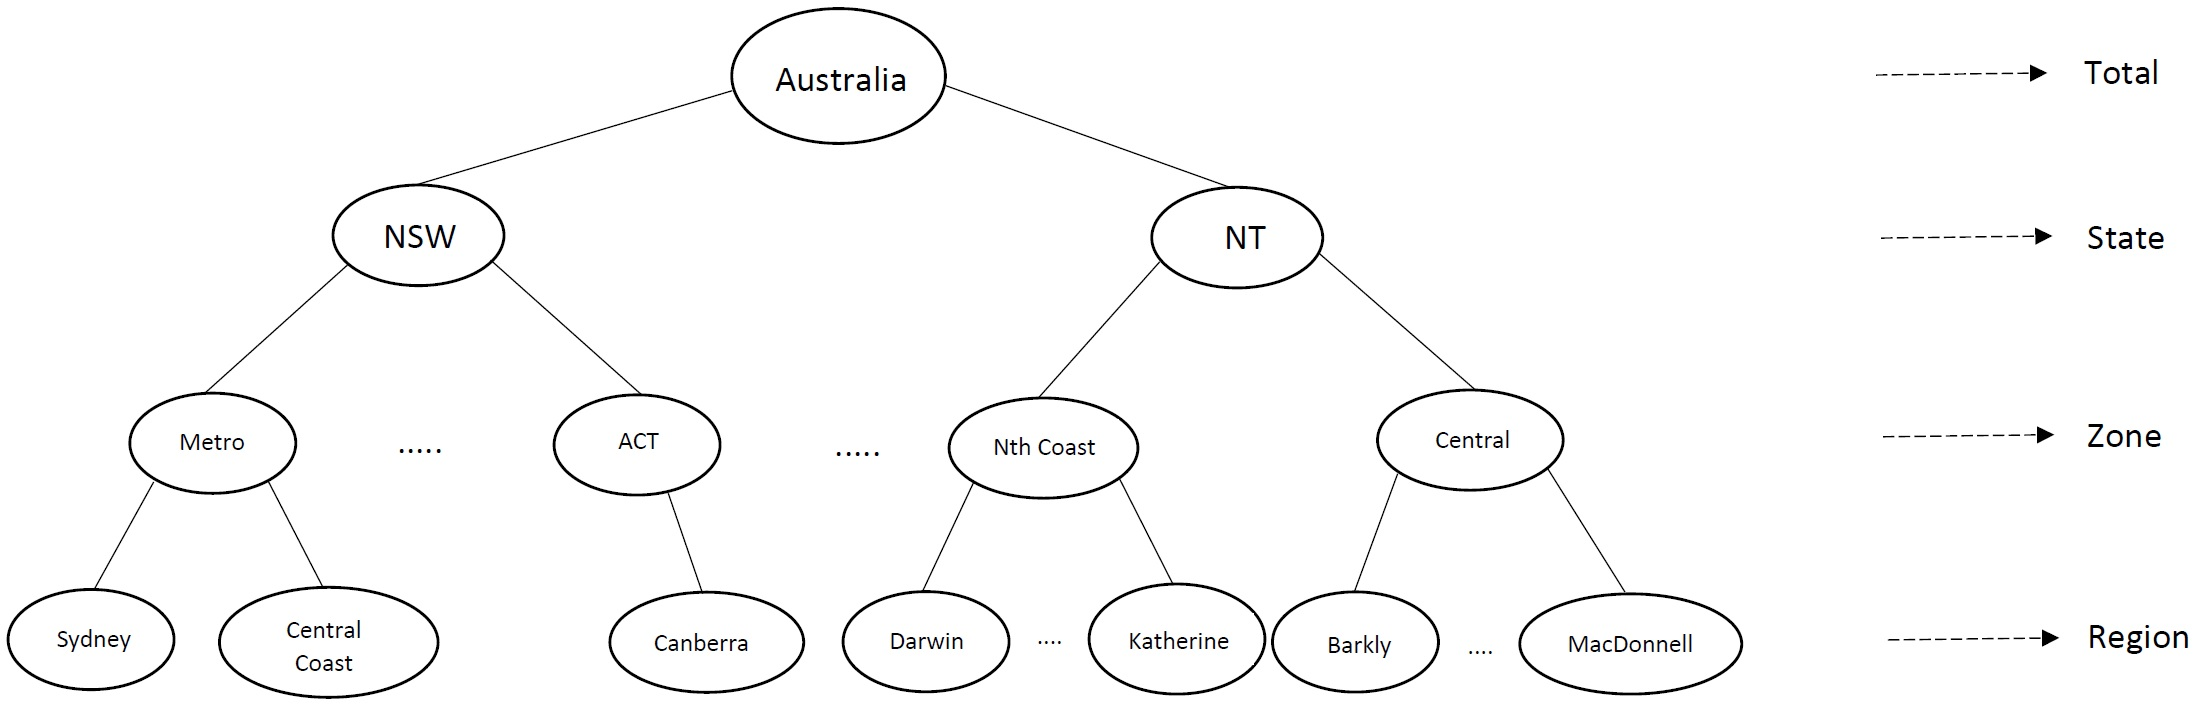
\includegraphics[width=450px,height=150px]{Paper-Figures/Australian_hierarchy_structure} 

}

\caption{Australian geographic hierarchical structure.}\label{fig:Australiahierarchystructure}
\end{figure}

\begin{figure}

{\centering 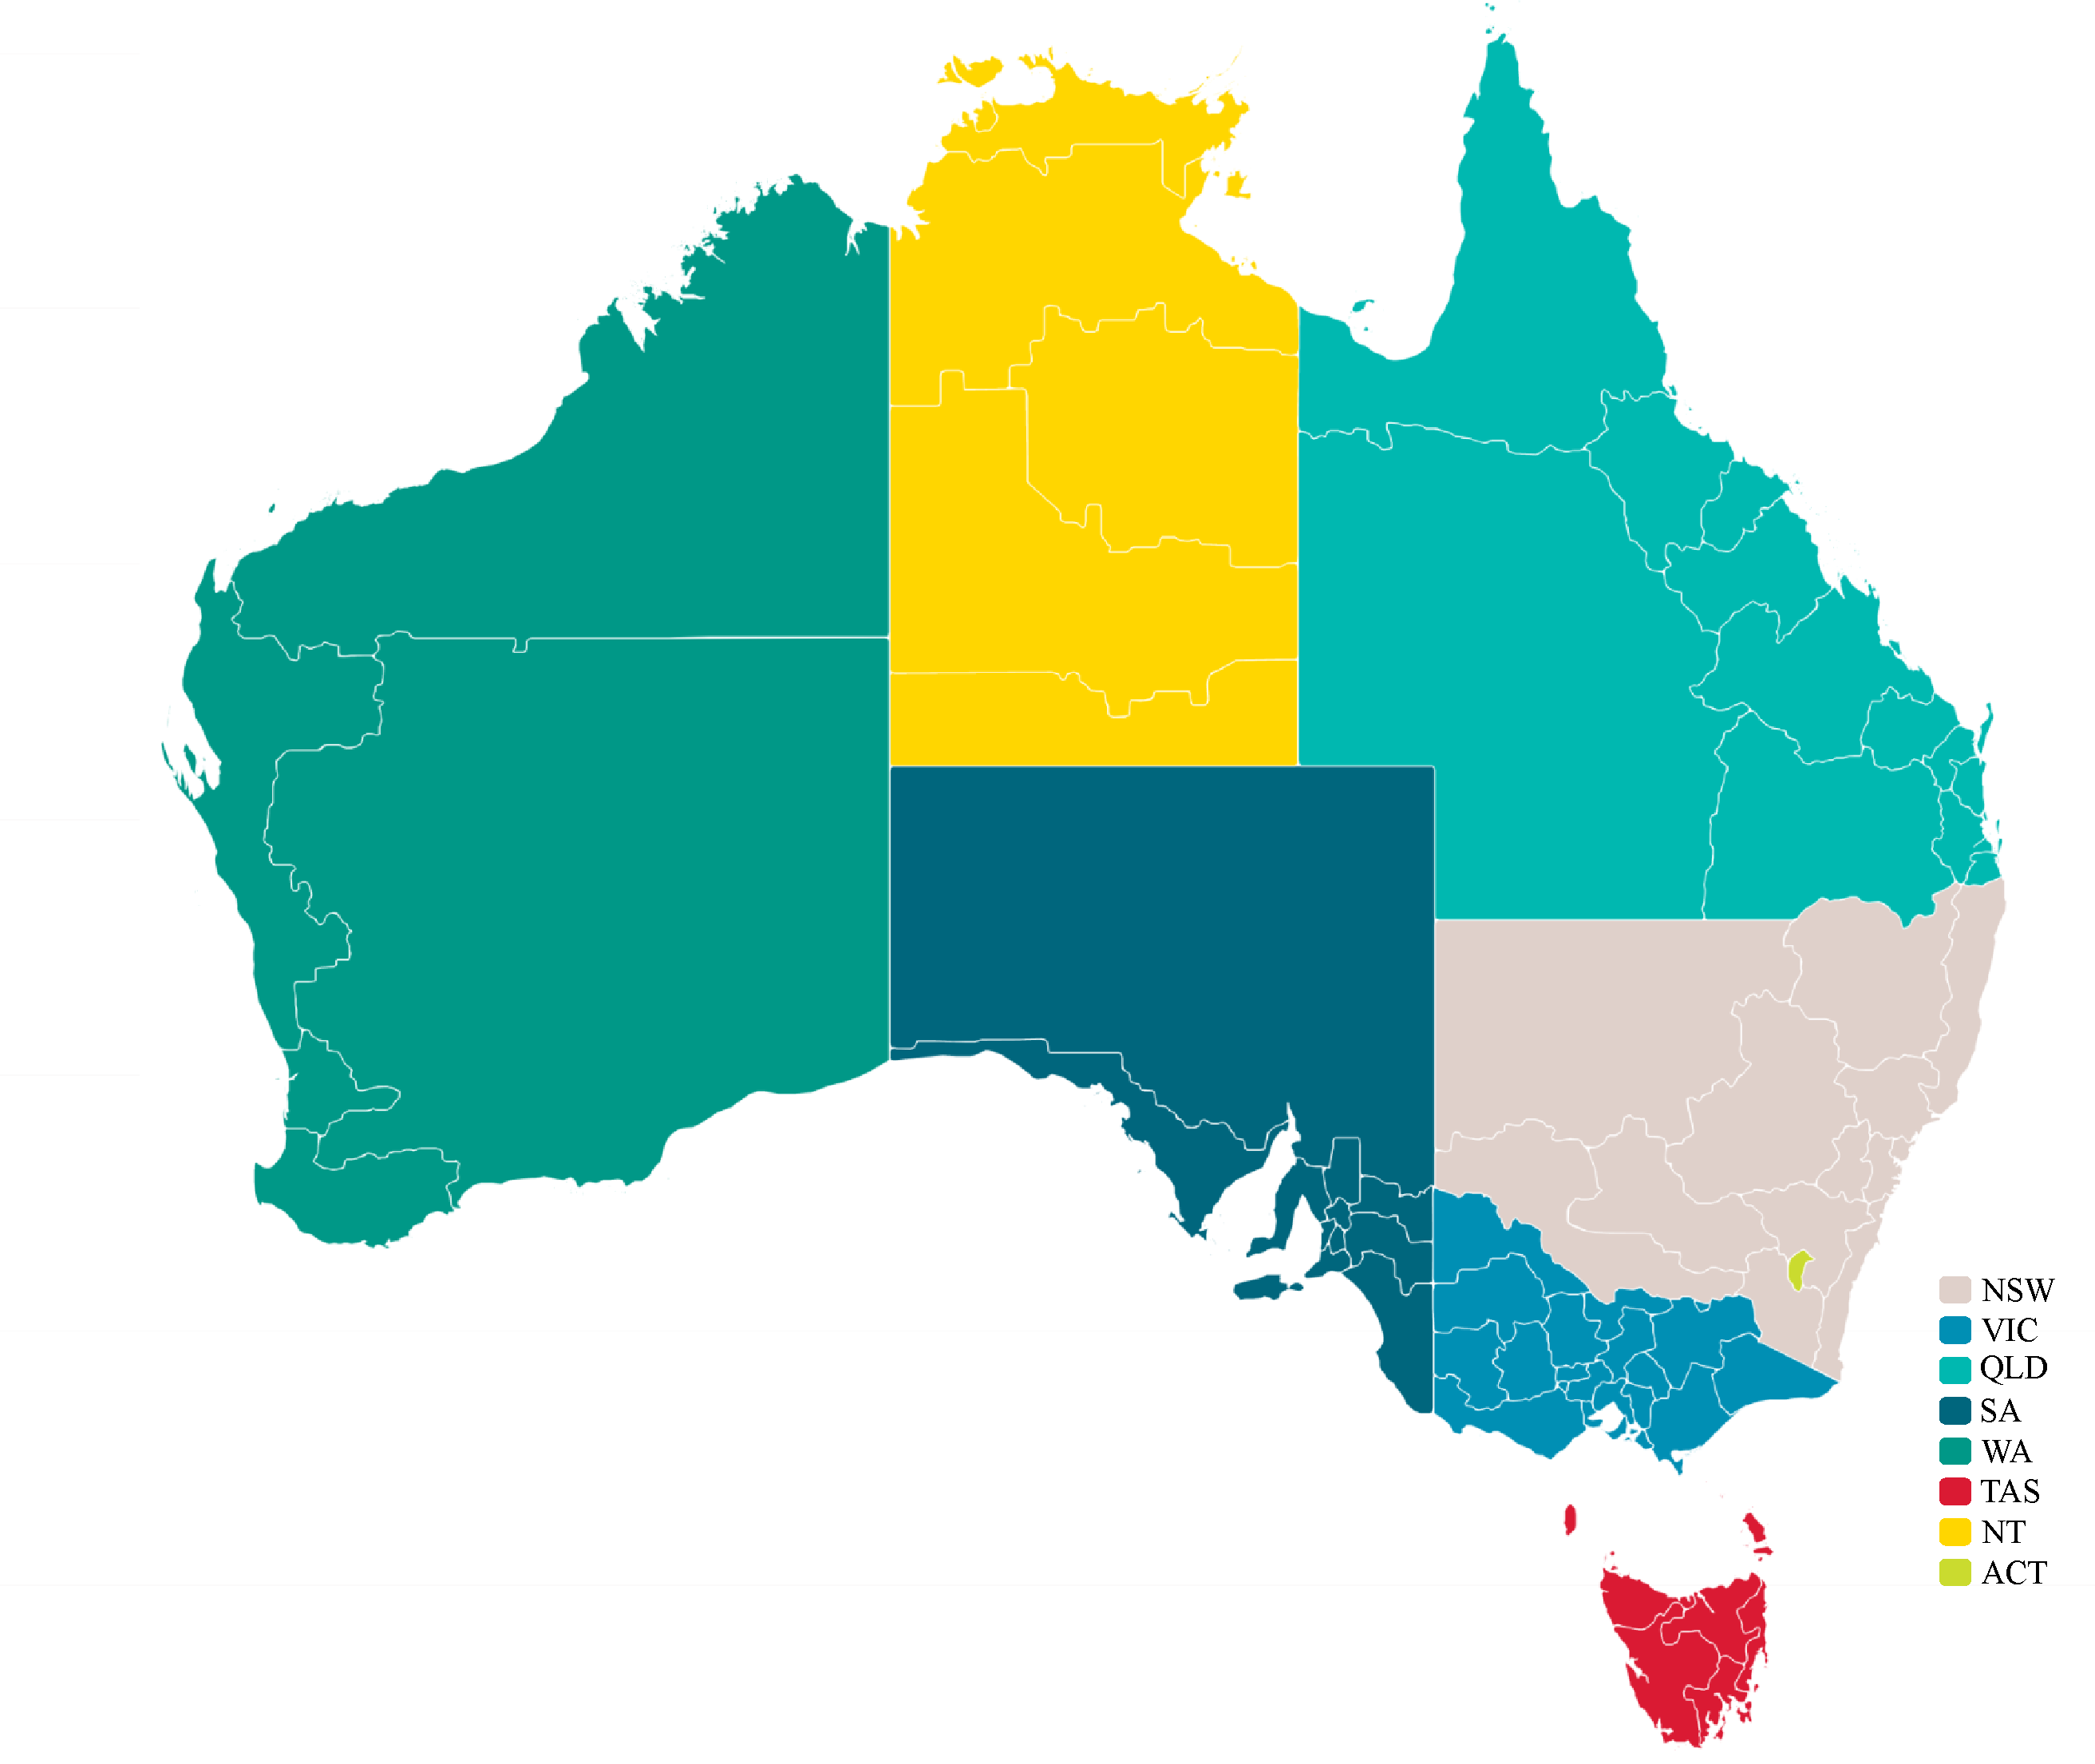
\includegraphics[width=450px,height=360px]{Paper-Figures/ausTurRegions} 

}

\caption{Australia tourism region map - colors represent states.}\label{fig:Australiahierarchystructuremap}
\end{figure}

\newpage

In this dataset we have three levels of geographic divisions in
Australia. In the first level, Australia is divided into seven `States'
including New South Wales (NSW), Victoria (VIC), Queensland (QLD), South
Australia (SA), Western Australia (WA), Tasmania (TAS) and Northern
Territory (NT). In the second and third levels, it is divided into 27
`Zones' and 76 `Regions' (for details about Australia geographic
divisions see Figure \ref{fig:Australiahierarchystructure} and Table
\ref{tab:Australiageographicaldivision} and also Figure
\ref{fig:Australiahierarchystructuremap} which shows Australia map
divided by tourism region and colored by states\footnote{For more
  information about the map:
  \url{https://www.tra.gov.au/tra/2016/Tourism_Region_Profiles/Region_profiles/index.html}}).

For `Purpose' we have four groups: Holiday (Hol), Visiting friends and
relatives (Vis), Business (Bus) and Other (Oth). Based on the geographic
hierarchy and purpose grouping, we end up with 8 hierarchical levels
with 555 series in total:

\begin{itemize}
\tightlist
\item
  Level 0 = Total for Australia
\item
  Level 1 = State totals
\item
  Level 2 = Zone totals
\item
  Level 3 = Region totals
\item
  Level 4 = Purpose totals
\item
  Level 5 = State \(\times\) Purpose totals
\item
  Level 6 = Zone \(\times\) Purpose totals
\item
  Level 7 = bottom level series
\end{itemize}

\begin{table}[!h]

\caption{\label{tab:Australiageographicalpurposedivision}Number of Australian domestic tourism series in each level of the hierarchy and group structure.}
\centering
\begin{tabular}{lrrr}
\toprule
Geographic division & \# series (geographic division) & \# series (purpose of travel) & Total\\
\midrule
Australia & 1 & 4 & 5\\
State & 7 & 28 & 35\\
Zone & 27 & 108 & 135\\
Region & 76 & 304 & 380\\
Total & 111 & 444 & 555\\
\bottomrule
\end{tabular}
\end{table}

We report the forecast results for all these hierarchical levels, as
well as the average RMSE across all the levels of the hierarchy. We used
different predictors in the OLS predictor matrix for the rolling and
fixed origin approaches. For the rolling origin model, we included a
linear trend, 11 dummy variables, and 12 lags. For the fixed origin
model, we included a quadratic trend, 11 dummy variables, and lags 1 and
12. This is intended to capture the monthly seasonality. In addition,
before running the model, we partition the data into training and test
sets, with the last 24 months (2 years) as our test set, and the rest as
our training set.

\begin{table}[!h]

\caption{\label{tab:Tourismdataresulrolling}Mean(RMSE) for ETS, ARIMA and OLS with and without reconciliation - Rolling origin 24-step-ahead - Tourism dataset}
\centering
\begin{tabular}{lrrrrrr}
\toprule
\multicolumn{1}{c}{} & \multicolumn{3}{c}{Unreconciled} & \multicolumn{3}{c}{Reconciled} \\
\cmidrule(l{2pt}r{2pt}){2-4} \cmidrule(l{2pt}r{2pt}){5-7}
Level & ETS & ARIMA & OLS & ETS & ARIMA & OLS\\
\midrule
Level 0 & 1516.4 & 1445.5 & 1415.1 & 1533.6 & 1453.4 & 1454.4\\
Level 1 & 511.4 & 493.1 & 510.8 & 495.9 & 457.6 & 488.3\\
Level 2 & 214.8 & 219.0 & 224.5 & 209.2 & 207.5 & 212.4\\
Level 3 & 122.9 & 125.1 & 124.0 & 118.7 & 120.5 & 119.5\\
Level 4 & 676.0 & 709.2 & 694.5 & 668.3 & 679.7 & 678.5\\
Level 5 & 213.1 & 220.1 & 216.1 & 210.6 & 209.4 & 211.1\\
Level 6 & 97.5 & 102.4 & 101.0 & 96.4 & 99.8 & 98.6\\
Level 7 & 56.2 & 58.2 & 58.2 & 56.0 & 57.7 & 57.2\\
\bottomrule
\end{tabular}
\end{table}

\begin{table}[t]

\caption{\label{tab:TourismdataresultRMSE}Mean(RMSE) for ETS, ARIMA and OLS with and without reconciliation - Fixed origin 24-step-ahead - Tourism dataset}
\centering
\begin{tabular}{lrrrrrr}
\toprule
\multicolumn{1}{c}{} & \multicolumn{3}{c}{Unreconciled} & \multicolumn{3}{c}{Reconciled} \\
\cmidrule(l{2pt}r{2pt}){2-4} \cmidrule(l{2pt}r{2pt}){5-7}
Level & ETS & ARIMA & OLS & ETS & ARIMA & OLS\\
\midrule
Level 0 & 2238.6 & 3554.0 & 2528.9 & 2250.2 & 3179.4 & 2594.3\\
Level 1 & 593.6 & 570.1 & 596.5 & 553.8 & 626.3 & 587.2\\
Level 2 & 239.5 & 229.6 & 243.3 & 234.2 & 242.5 & 237.4\\
Level 3 & 132.6 & 129.4 & 127.1 & 126.7 & 129.4 & 124.6\\
Level 4 & 766.8 & 824.0 & 875.5 & 795.5 & 958.2 & 868.5\\
Level 5 & 226.7 & 241.2 & 236.7 & 222.5 & 236.9 & 230.7\\
Level 6 & 103.0 & 105.4 & 104.9 & 102.0 & 103.9 & 103.2\\
Level 7 & 59.1 & 58.8 & 58.6 & 58.5 & 58.7 & 58.0\\
\bottomrule
\end{tabular}
\end{table}

In Tables \ref{tab:Tourismdataresulrolling} and
\ref{tab:TourismdataresultRMSE}, we show the average RMSE for the
1-month and 24-month forecasts. Methods include ETS, ARIMA and our
proposed OLS forecasting model. In Table
\ref{tab:Tourismdataresulrolling} we forecast 24 periods ahead by
computing rolling origin forecasts, rolling forward month by month. In
Table \ref{tab:TourismdataresultRMSE} we generate fixed origin
24-step-ahead forecasts. In these tables we show forecasts with and
without reconciliation.

These results show that our proposed OLS forecasting model produces
forecast accuracy similar to ETS and ARIMA, which are computationally
heavy for many time series. Also they show the usefulness of the
reconciliation in decreasing the average RMSE in all the three methods.
Except for the total series, reconciliation can help in forecasting all
the hierarchical levels. Also, because the higher level series have
higher counts, the errors are larger in magnitude (see Figures
\ref{fig:boxplotrollingtourism} and \ref{fig:boxplottourism}). To better
compare errors across all the hierarchy levels we scaled the errors (See
\protect\hyperlink{appendixA}{Appendix A}).

In Figures \ref{fig:boxplotrollingtourism} and \ref{fig:boxplottourism}
we display the error box plots for both reconciled and unreconciled
forecasts using all three methods, for 1-step ahead and 24-steps ahead.
In these figures we can visualize the error distributions across all the
models, as well as the usefulness of the reconciliation step in
improving the forecasts. In particular, we see that as expected by
applying rolling origin 24-step-ahead forecasts, the error densities are
closer and more distributed around zero than the fixed origin
24-step-ahead forecasts.

Figures \ref{fig:forecstrolling24tourismtotal} and
\ref{fig:forecstrolling24tourism} show the rolling and fixed origin
24-step-ahead forecast results for the total series and one of the
bottom level series, `BACBus' (Geelong - Business). In these plots we
have both reconciled (solid lines) and unreconciled (dashed lines)
forecasts and we see that the reconciliation step improves the forecasts
in this series. We also see that the OLS model forecast accuracy is
similar to the other two methods.

\begin{figure}

{\centering \includegraphics[width=1\linewidth]{hcf_files/figure-latex/boxplotrollingtourism-1} 

}

\caption{Box plots of forecast errors from reconciled and unreconciled ETS, ARIMA and OLS methods at each hierarchical level for rolling origin 24-step-ahead tourism demand.}\label{fig:boxplotrollingtourism}
\end{figure}

\begin{figure}

{\centering \includegraphics[width=1\linewidth]{hcf_files/figure-latex/boxplottourism-1} 

}

\caption{Box plots of forecast errors for reconciled and unreconciled ETS, ARIMA and OLS methods at each hierarchical level for fixed origin 24-step-ahead tourism demand.}\label{fig:boxplottourism}
\end{figure}

\begin{figure}

{\centering \includegraphics[width=1\linewidth]{hcf_files/figure-latex/forecstrolling24tourismtotal-1} 

}

\caption{The actual test set for the 'Total series' compared to the forecasts from reconciled and unreconciled ETS, ARIMA and OLS methods for rolling and fixed origin 24-step-ahead tourism demand.}\label{fig:forecstrolling24tourismtotal}
\end{figure}

\begin{figure}

{\centering 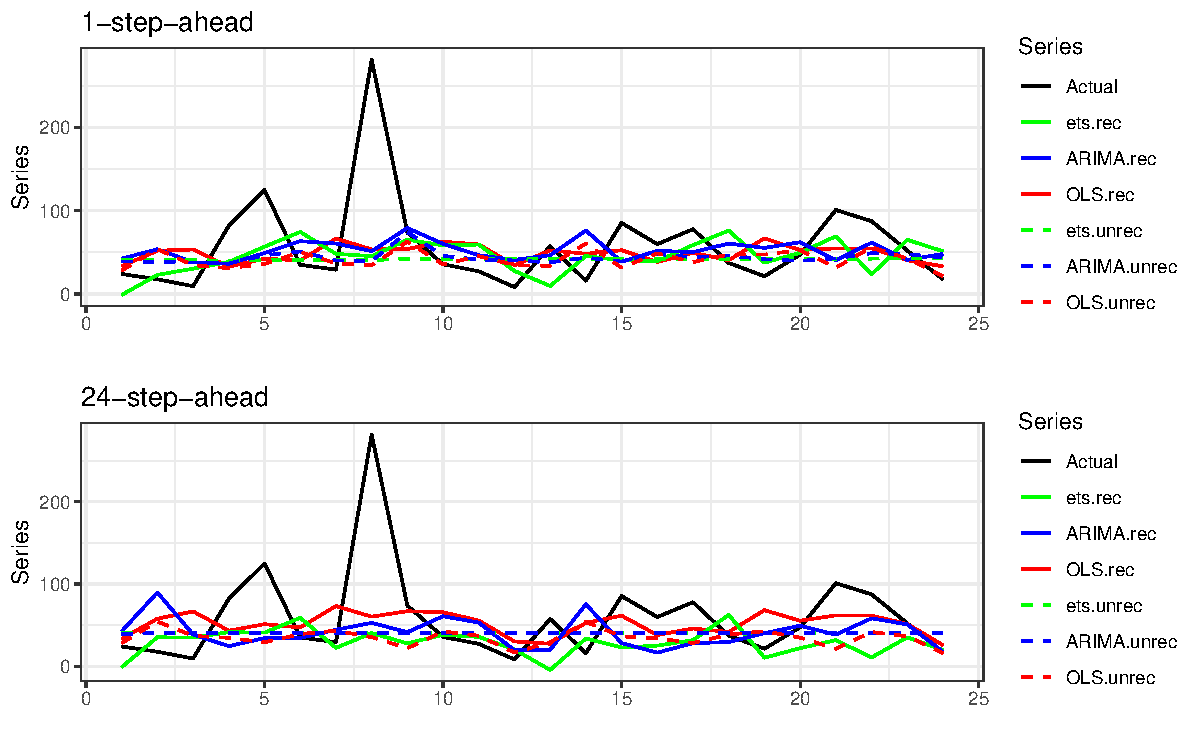
\includegraphics[width=1\linewidth]{hcf_files/figure-latex/forecstrolling24tourism-1} 

}

\caption{The actual test set for the 'BACBus' bottom level series compared to the forecasts from reconciled and unreconciled ETS, ARIMA and OLS methods for rolling and fixed origin 24-step-ahead tourism demand.}\label{fig:forecstrolling24tourism}
\end{figure}

\newpage

Table \ref{tab:Tourismdatacomputationtime} compares the computation time
of the three methods for rolling and fixed origin 24-step-ahead
forecasting. We see that the OLS forecasting model is much faster
compared to the other methods. Also, since reconciliation is a linear
process, in all methods it is very fast and does not affect computation
time significantly.

\begin{table}[t]

\caption{\label{tab:Tourismdatacomputationtime}Computation time (seconds) for ETS, ARIMA and OLS with and without reconciliation - Rolling and fixed origin 24-step-ahead - Tourism dataset}
\centering
\begin{tabular}{>{\raggedright\arraybackslash}p{3cm}>{\raggedleft\arraybackslash}p{3cm}>{\raggedleft\arraybackslash}p{3cm}rr}
\toprule
\multicolumn{1}{c}{} & \multicolumn{2}{c}{Rolling origin} & \multicolumn{2}{c}{Fixed origin} \\
\cmidrule(l{2pt}r{2pt}){2-3} \cmidrule(l{2pt}r{2pt}){4-5}
 & Unreconciled & Reconciled & Unreconciled & Reconciled\\
\midrule
ETS & 10924.57 & 10924.60 & 407.10 & 407.15\\
ARIMA & 31146.38 & 31146.52 & 1116.15 & 1116.19\\
OLS & 48.40 & 48.31 & 17.42 & 17.80\\
\bottomrule
\end{tabular}
\end{table}

Since we are using a linear model, we can easily include exogenous
variables which can often be helpful in improving forecast accuracy. In
this application, we tried including an ``Easter'' dummy variable
indicating the timing of Easter, but its affect on forecast accuracy was
minimal, so it was omitted in the model reported here.

\FloatBarrier

\hypertarget{wikipedia-pageviews-grouped-structure}{%
\subsection{Wikipedia pageviews: Grouped
structure}\label{wikipedia-pageviews-grouped-structure}}

The second dataset consists of one year of daily data (2016-06-01 to
2017-06-29) on Wikipedia pageviews for the most popular social networks
articles \autocite{ashouri2018}. This dataset is noisier compared with
the Australian monthly tourism data and forecasting its series is more
challenging. It has a grouped structure, with grouping attributes:
`Agent': Spider, User, `Access': Desktop, Mobile app, Mobile web,
`Language': en (English), de (German), es (Spanish), zh (Chinese) and
`Purpose': Blogging related, Business, Gaming, General purpose, Life
style, Photo sharing, Reunion, Travel, Video (check Table
\ref{tab:wikipediagroupingstructure}). We display the group structure in
Table \ref{tab:wikipediagroupingstructure} and Figure
\ref{fig:wikigroupstructure}. In Figure \ref{fig:wikigroupstructure} we
use one possible hierarchy for this dataset, but the order of the
hierarchy can be switched. The final dataset includes 913 time series,
each with length 394. The group structure and different levels include:

\begin{itemize}
\tightlist
\item
  Level 0 = Total
\item
  Level 1 = Agent
\item
  Level 2 = Access
\item
  Level 3 = Language
\item
  Level 4 = Purpose
\item
  Level 5 = bottom level series
\end{itemize}

For this daily dataset, in the OLS forecasting model we include in the
predictor matrix a quadratic trend, 6 seasonal dummies and all 7 lags
for rolling, and for fixed origin model we use a quadratic trend, 6
seasonal dummies and lags 1 and 7. We partitioned the data into two
parts training and test sets. We used the last 28 days for our test set
and the rest for the training set.

\begin{table}[t]

\caption{\label{tab:wikipediagroupingstructure}Social networking Wikipedia article grouping structure}
\centering
\begin{tabular}{llll}
\toprule
Grouping & Series & Grouping & Series\\
\midrule
Total &  & Language & \\
 & 1. Social Network &  & 10. zh (Chinese)\\
Agent &  & Purpose & \\
 & 2. Spider &  & 11. Blogging related\\
 & 3. User &  & 12. Business\\
Access &  &  & 13. Gaming\\
 & 4. Desktop &  & 14. General purpose\\
 & 5. Mobile app &  & 15. Life style\\
 & 6. Mobile web &  & 16. Photo sharing\\
Language &  &  & 17. Reunion\\
 & 7. en (English) &  & 18. Travel\\
 & 8. de (German) &  & 19. Video\\
 & 9. es (Spanish) &  & \\
\bottomrule
\end{tabular}
\end{table}

\begin{figure}

{\centering 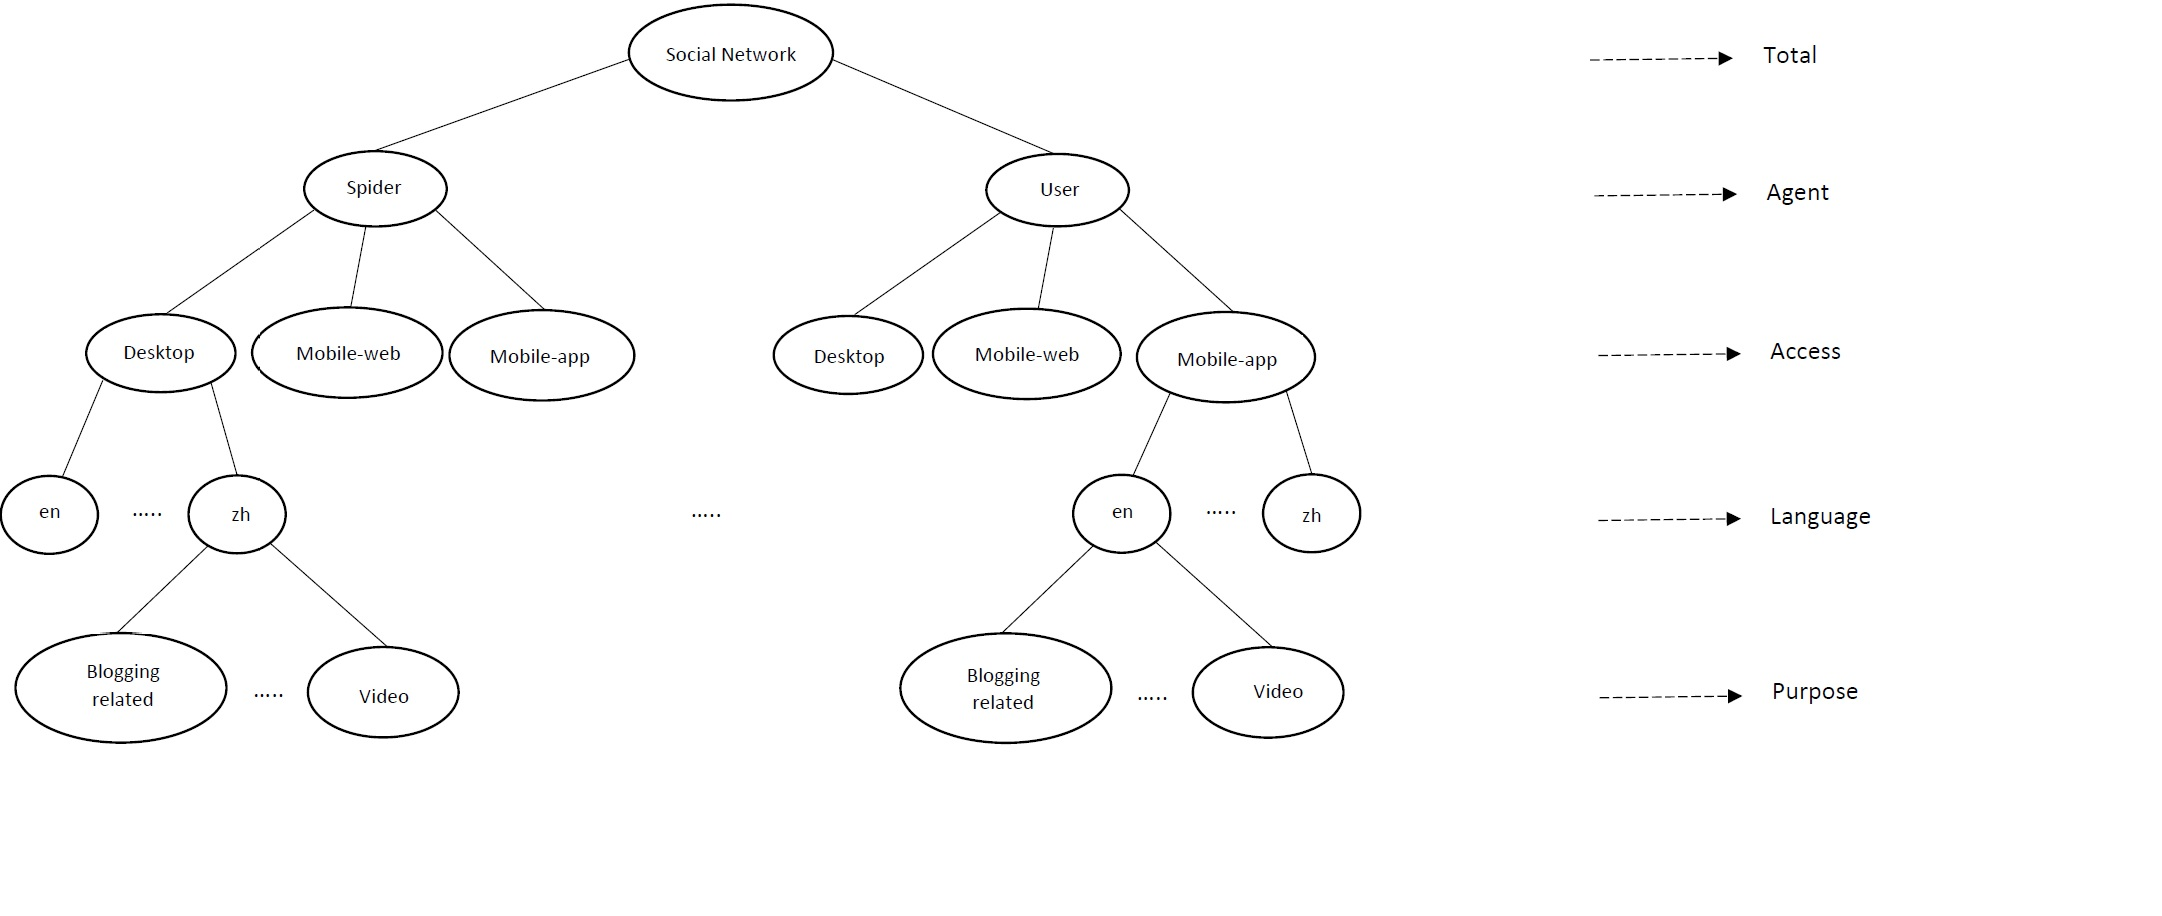
\includegraphics[width=500px,height=250px]{Paper-Figures/Wiki_group_structure} 

}

\caption{One of the possible hierarchical structures for the Wikipedia pageview dataset.}\label{fig:wikigroupstructure}
\end{figure}

Table \ref{tab:wikipediadataresulrolling},
\ref{tab:wikipediadataresultRMSE} and
\ref{tab:wikipediadatacomputationtime} represent the RMSE results and
computation time. Although these time series are noisier, we still get
acceptable results for the OLS forecasting model compared with ETS and
ARIMA. In this case, we get similar results with and without the
reconciliation step.

Figures \ref{fig:boxplotrollingwiki} and \ref{fig:boxplotwiki} display
the forecast error box plot. These plots are for rolling and fixed
origin 28-step-ahead forecasts in each level of grouping. Further, we
can see that the error distribution is almost similar in all levels
across the different methods. The only exception is the Total series,
where ETS performs significantly better than ARIMA and OLS. We also note
that the reconciliation is less effective. As in the tourism example, in
higher levels, series have higher counts and therefore their error
magnitudes are larger.

\begin{table}[!h]

\caption{\label{tab:wikipediadataresulrolling}Mean(RMSE) for ETS, ARIMA and OLS with and without reconciliation - Rolling origin 28-step-ahead - Wikipedia dataset}
\centering
\begin{tabular}{lrrrrrr}
\toprule
\multicolumn{1}{c}{} & \multicolumn{3}{c}{Unreconciled} & \multicolumn{3}{c}{Reconciled} \\
\cmidrule(l{2pt}r{2pt}){2-4} \cmidrule(l{2pt}r{2pt}){5-7}
Level & ETS & ARIMA & OLS & ETS & ARIMA & OLS\\
\midrule
Level 0 & 10773.7 & 15060.7 & 12288.0 & 11014.7 & 14276.5 & 12010.0\\
Level 1 & 8272.9 & 10196.3 & 8564.0 & 7736.9 & 9904.1 & 8518.0\\
Level 2 & 6524.7 & 6705.0 & 5915.5 & 6257.4 & 7142.5 & 6100.4\\
Level 3 & 4870.1 & 6333.0 & 5612.5 & 4981.9 & 6370.0 & 5633.6\\
Level 4 & 5233.5 & 4659.5 & 3935.9 & 5001.4 & 4586.5 & 3900.7\\
Level 5 & 358.1 & 239.0 & 258.2 & 362.2 & 241.6 & 258.6\\
\bottomrule
\end{tabular}
\end{table}

\begin{table}[t]

\caption{\label{tab:wikipediadataresultRMSE}Mean(RMSE) for ETS, ARIMA and OLS with and without reconciliation - Fixed origin 28-step-ahead - Wikipedia dataset}
\centering
\begin{tabular}{lrrrrrr}
\toprule
\multicolumn{1}{c}{} & \multicolumn{3}{c}{Unreconciled} & \multicolumn{3}{c}{Reconciled} \\
\cmidrule(l{2pt}r{2pt}){2-4} \cmidrule(l{2pt}r{2pt}){5-7}
Level & ETS & ARIMA & OLS & ETS & ARIMA & OLS\\
\midrule
Level 0 & 14846.9 & 24298.8 & 20203.7 & 14999.2 & 24649.9 & 19978.0\\
Level 1 & 13608.7 & 17277.0 & 14985.7 & 12240.3 & 16810.5 & 14894.2\\
Level 2 & 7117.4 & 10732.0 & 8866.4 & 7523.4 & 11068.8 & 8938.5\\
Level 3 & 6475.9 & 9580.4 & 7913.7 & 6509.0 & 9799.1 & 8078.9\\
Level 4 & 5302.7 & 8611.3 & 5694.1 & 5307.3 & 8239.8 & 5688.7\\
Level 5 & 435.6 & 389.4 & 363.7 & 437.7 & 391.2 & 363.5\\
\bottomrule
\end{tabular}
\end{table}

\begin{figure}

{\centering \includegraphics[width=1\linewidth]{hcf_files/figure-latex/boxplotrollingwiki-1} 

}

\caption{Box plots of forecast errors for reconciled and unreconciled ETS, ARIMA and OLS methods at each hierarchical level for rolling origin 28-step-ahead Wikipedia pageviews.}\label{fig:boxplotrollingwiki}
\end{figure}

\begin{figure}

{\centering \includegraphics[width=1\linewidth]{hcf_files/figure-latex/boxplotwiki-1} 

}

\caption{Box plots of forecast errors for reconciled and unreconciled ETS, ARIMA and OLS methods at each hierarchical level for fixed origin 28-step-ahead Wikipedia pageviews.}\label{fig:boxplotwiki}
\end{figure}

In Figures \ref{fig:forecstrolling28wikitotal} and
\ref{fig:forecstrolling28wiki}, we display results for the total and one
of the bottom level series, `desktopusenPho' (desktop-user-english-photo
sharing). The plot shows rolling and fixed origin 28-step-ahead forecast
results for ETS, ARIMA and OLS, with (solid lines) and without (dashed
lines) applying reconciliation. We see that the OLS forecasting model
performs close to the other two methods, and reconciliation improves the
forecasts.

\begin{figure}

{\centering \includegraphics[width=1\linewidth]{hcf_files/figure-latex/forecstrolling28wikitotal-1} 

}

\caption{The actual test set for the 'Total' series compared to the forecasts from reconciled and unreconciled ETS, ARIMA and OLS methods for rolling and fixed origin 28-step-ahead Wikipedia pageviews.}\label{fig:forecstrolling28wikitotal}
\end{figure}

\begin{figure}

{\centering 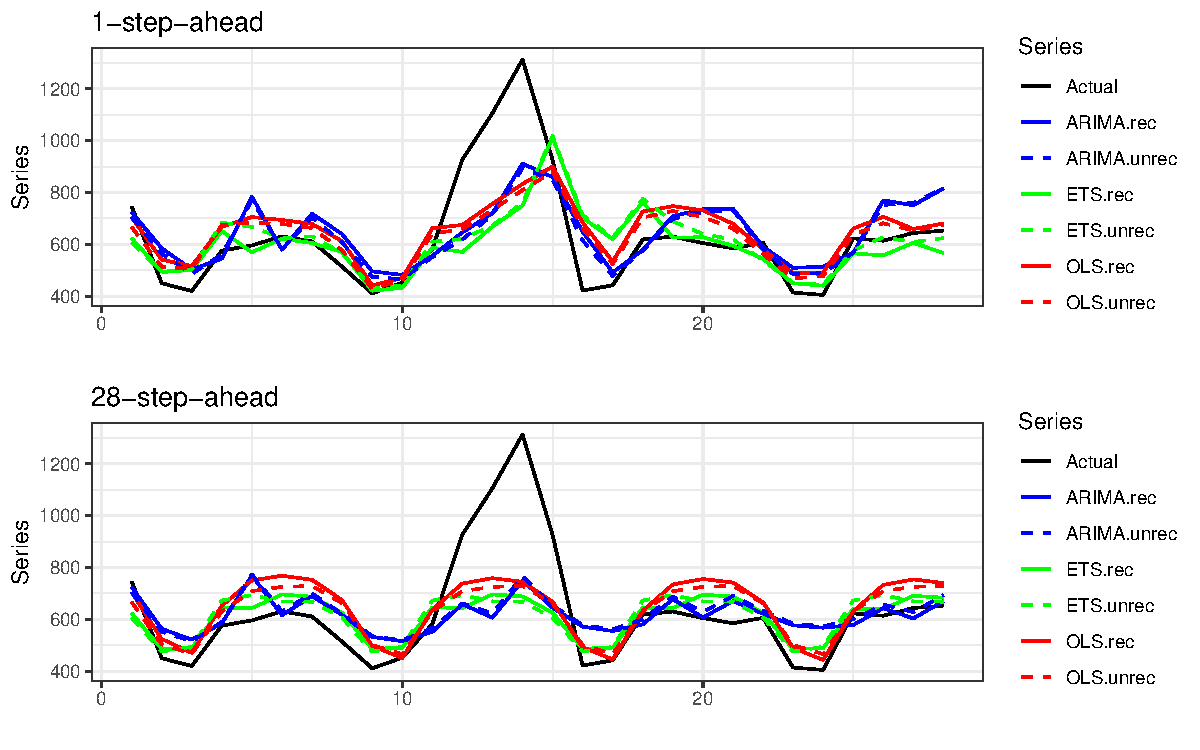
\includegraphics[width=1\linewidth]{hcf_files/figure-latex/forecstrolling28wiki-1} 

}

\caption{The actual test set for the 'desktopusenPho21' bottom level series compared to the forecasts from reconciled and unreconciled ETS, ARIMA and OLS methods for rolling and fixed origin 28-step-ahead Wikipedia pageviews.}\label{fig:forecstrolling28wiki}
\end{figure}

Lastly, Table \ref{tab:wikipediadatacomputationtime} presents the
computation times for all three methods. ETS and ARIMA are clearly much
more computationally heavy compared with OLS. As in the Australian
tourism dataset, running reconciliation does not have much effect on
computation time.

\begin{table}[t]

\caption{\label{tab:wikipediadatacomputationtime}Computation time (seconds) for ETS, ARIMA and OLS with and without reconciliation - Rolling and fixed origin 28-step-ahead - Wikipedia dataset}
\centering
\begin{tabular}{>{\centering\arraybackslash}p{3cm}>{\centering\arraybackslash}p{3cm}>{\centering\arraybackslash}p{3cm}cc}
\toprule
\multicolumn{1}{c}{} & \multicolumn{4}{c}{Computation time (secs)} \\
\cmidrule(l{2pt}r{2pt}){2-5}
\multicolumn{1}{c}{} & \multicolumn{2}{c}{Rolling origin} & \multicolumn{2}{c}{Fixed origin} \\
\cmidrule(l{2pt}r{2pt}){2-3} \cmidrule(l{2pt}r{2pt}){4-5}
 & Unreconciled & Reconciled & Unreconciled & Reconciled\\
\midrule
ETS & 13963.93 & 13963.96 & 450.89 & 450.92\\
ARIMA & 10327.02 & 10327.15 & 670.40 & 670.44\\
OLS & 82.55 & 82.62 & 35.39 & 35.43\\
\bottomrule
\end{tabular}
\end{table}

\hypertarget{conclusion}{%
\section{Conclusion}\label{conclusion}}

We proposed a linear model approach to forecast hierarchical or grouped
time series in a much faster way, but with accuracy that nearly matches
that of forecast methods such as ETS and ARIMA. This is especially
useful in large collections of time series, as is typical in
hierarchical and grouped structures. Although ETS and ARIMA are
advantageous in terms of forecasting power and accuracy, they can be
computationally heavy when facing large collections of time series in
the hierarchy. Adding another faster option for calculating base
forecasts was our purpose in this research. Here we suggest a linear
model, OLS, instead of ETS and ARIMA which is not computationally
intensive. We also showed that OLS can compete with ETS and ARIMA in
terms of forecasting accuracy. An important feature of our model is its
ability to easily include external information such as holiday dummies
or other external series. We also note that OLS has the additional
practical advantage of handling missing data while ETS and ARIMA require
imputation. In literature \textcite{pennings2017} is one example for
forecasting hierarchical series. This method is applying state space
models and although it is flexible in handling outliers, missing data
and external features it is less flexible to different kinds of datasets
and it is computationally more complex. In addition to the computation
adjustment, since our proposed approach is computationally cheap it is
especially useful for model selection.

\hypertarget{acknowledgements}{%
\section*{Acknowledgements}\label{acknowledgements}}
\addcontentsline{toc}{section}{Acknowledgements}

The first and third authors of this research were partially funded by
Ministry of Science and Technology (MOST), Taiwan {[}Grant
106-2420-H-007-019{]}.

\clearpage

\hypertarget{appendixA}{%
\section*{Appendix A}\label{appendixA}}
\addcontentsline{toc}{section}{Appendix A}

We provide boxplots of the scaled forecasted errors for the tourism
example. These plots are displayed for both rolling forward and
multiple-step-ahead forecasts.

\begin{figure}

{\centering \includegraphics[width=0.88\linewidth]{hcf_files/figure-latex/boxplotrollingtourismappendix-1} 

}

\caption{Box plots of scaled forecast errors from reconciled and unreconciled ETS, ARIMA and OLS methods at each hierarchical level for rolling origin 24-step-ahead tourism demand.}\label{fig:boxplotrollingtourismappendix}
\end{figure}

\begin{figure}

{\centering \includegraphics[width=0.88\linewidth]{hcf_files/figure-latex/boxplottourismappendix-1} 

}

\caption{Box plots of scaled forecast errors from reconciled and unreconciled ETS, ARIMA and OLS methods at each hierarchical level for fixed origin 24-step-ahead tourism demand.}\label{fig:boxplottourismappendix}
\end{figure}

\clearpage

\clearpage

\hypertarget{appendixB}{%
\section*{Appendix B}\label{appendixB}}
\addcontentsline{toc}{section}{Appendix B}

In Figure \ref{fig:loopsvsmatrix}, we compare the forecasts obtained
using separate regression models versus matrix computation for the
Australian domestic tourism example. Although mathematically both
approaches should yield the same results, the results in practice are
slightly different due to numerical deviations. Table
\ref{tab:Tourismdatacomputationtimeappendix} shows the matrix approach
is computationally heavier due to greater memory requirements.

\begin{figure}

{\centering \includegraphics[width=1\linewidth]{hcf_files/figure-latex/loopsvsmatrix-1} 

}

\caption{Comparison of the forecasts obtained  using a matrix approach and separate regression models to reconcile forecasts for rolling and fixed origin 24-step-ahead tourism demand (bottom level series only).}\label{fig:loopsvsmatrix}
\end{figure}

\begin{table}[t]

\caption{\label{tab:Tourismdatacomputationtimeappendix}Computation time (seconds) for OLS using the matrix approach and separate regression models, with and without reconciliation, on a rolling and fixed origin for 24 steps ahead, using the tourism dataset.}
\centering
\begin{tabular}{>{\raggedright\arraybackslash}p{3cm}>{\raggedleft\arraybackslash}p{3cm}>{\raggedleft\arraybackslash}p{3cm}rr}
\toprule
\multicolumn{1}{c}{} & \multicolumn{2}{c}{Rolling origin} & \multicolumn{2}{c}{Fixed origin} \\
\cmidrule(l{2pt}r{2pt}){2-3} \cmidrule(l{2pt}r{2pt}){4-5}
 & Unreconciled & Reconciled & Unreconciled & Reconciled\\
\midrule
Matrix approach & 202.06 & 209.84 & 87.73 & 105.69\\
Separate models & 48.40 & 48.31 & 16.66 & 16.85\\
\bottomrule
\end{tabular}
\end{table}

\clearpage

\hypertarget{appendixC}{%
\section*{Appendix C}\label{appendixC}}
\addcontentsline{toc}{section}{Appendix C}

In Figure \ref{fig:boxplotrollingtourismweight} and
\ref{fig:boxplottourismwight} we display a box plot comparison of the
results using two different reconciliation functions, weighted and
unweighted (Equations \eqref{eq:initialW} and \eqref{eq:mint}), for ETS,
ARIMA and the proposed OLS methods. We can see that for the base level
the unweighted approach is similar, but for some lower levels the
weighted approach provides more accurate forecasts.

\begin{figure}

{\centering \includegraphics[width=1\linewidth]{hcf_files/figure-latex/boxplotrollingtourismweight-1} 

}

\caption{Box plots of forecast errors from OLS and WLS reconciled ETS, ARIMA and OLS methods at each hierarchical level for rolling origin 24-step-ahead tourism demand.}\label{fig:boxplotrollingtourismweight}
\end{figure}

\begin{figure}

{\centering \includegraphics[width=1\linewidth]{hcf_files/figure-latex/boxplottourismwight-1} 

}

\caption{Box plots of forecast errors from OLS and WLS reconciled ETS, ARIMA and OLS methods at each hierarchical level for fixed origin 24-step-ahead tourism demand.}\label{fig:boxplottourismwight}
\end{figure}

\clearpage

\printbibliography

\end{document}
